% !TeX document-id = {fd3a097d-8ca3-4154-98bc-98947b5e5311}
% !TeX TXS-program:compile = txs:///pdflatex/[--shell-escape]
% !TEX root = master.tex
% !TeX encoding = UTF-8
% !TeX spellcheck = en_GB

\documentclass[10pt]{article}
%\documentclass[journal]{IEEEtran}
%\documentclass{report}
%\documentclass{ActaOulu}

\usepackage{graphicx}
\usepackage{listings}
\usepackage{amsmath}
\usepackage{systeme}
\usepackage{pdfpages}
\usepackage{float}
\usepackage{multicol}
\usepackage{titlesec}
%\usepackage[algo2e]{algorithm2e}
%\usepackage{algorithm}
%\usepackage{minted}
\usepackage{caption}
\usepackage[hidelinks]{hyperref}
\usepackage[a4paper, textwidth=470pt, textheight=750pt]{geometry}
\hypersetup{
	colorlinks=true,
	linkcolor=blue,     
	urlcolor=black,
	citecolor=blue,
	pdftitle={Evaluation of a blockchain platform: Ethereum}
}
\captionsetup{
	justification=raggedright,
	singlelinecheck=false
}
\graphicspath{ {./img/} }
\setlength{\columnsep}{0.6cm}
\addtolength{\skip\footins}{2pc plus 5pt} % footnote separation
\titlespacing\section{0pt}{22pt plus 4pt minus 2pt}{7pt plus 2pt minus 2pt}
\setlength\parindent{0pt} %noindent
% Copyright 2017 Sergei Tikhomirov, MIT License
% https://github.com/s-tikhomirov/solidity-latex-highlighting/

\usepackage{listings, xcolor}

\definecolor{verylightgray}{rgb}{.97,.97,.97}

\lstdefinelanguage{Solidity}{
	keywords=[1]{anonymous, assembly, assert, balance, break, call, callcode, case, catch, class, constant, continue, constructor, contract, debugger, default, delegatecall, delete, do, else, emit, event, experimental, export, external, false, finally, for, function, gas, if, implements, import, in, indexed, instanceof, interface, internal, is, length, library, log0, log1, log2, log3, log4, memory, modifier, new, payable, pragma, private, protected, public, pure, push, require, return, returns, revert, selfdestruct, send, solidity, storage, struct, suicide, super, switch, then, this, throw, transfer, true, try, typeof, using, value, view, while, with, addmod, ecrecover, keccak256, mulmod, ripemd160, sha256, sha3}, % generic keywords including crypto operations
	keywordstyle=[1]\color{blue}\bfseries,
	keywords=[2]{address, bool, byte, bytes, bytes1, bytes2, bytes3, bytes4, bytes5, bytes6, bytes7, bytes8, bytes9, bytes10, bytes11, bytes12, bytes13, bytes14, bytes15, bytes16, bytes17, bytes18, bytes19, bytes20, bytes21, bytes22, bytes23, bytes24, bytes25, bytes26, bytes27, bytes28, bytes29, bytes30, bytes31, bytes32, enum, int, int8, int16, int24, int32, int40, int48, int56, int64, int72, int80, int88, int96, int104, int112, int120, int128, int136, int144, int152, int160, int168, int176, int184, int192, int200, int208, int216, int224, int232, int240, int248, int256, mapping, string, uint, uint8, uint16, uint24, uint32, uint40, uint48, uint56, uint64, uint72, uint80, uint88, uint96, uint104, uint112, uint120, uint128, uint136, uint144, uint152, uint160, uint168, uint176, uint184, uint192, uint200, uint208, uint216, uint224, uint232, uint240, uint248, uint256, var, void, ether, finney, szabo, wei, days, hours, minutes, seconds, weeks, years},	% types; money and time units
	keywordstyle=[2]\color{teal}\bfseries,
	keywords=[3]{block, blockhash, coinbase, difficulty, gaslimit, number, timestamp, msg, data, gas, sender, sig, value, now, tx, gasprice, origin},	% environment variables
	keywordstyle=[3]\color{violet}\bfseries,
	identifierstyle=\color{black},
	sensitive=false,
	comment=[l]{//},
	morecomment=[s]{/*}{*/},
	commentstyle=\color{gray}\ttfamily,
	stringstyle=\color{red}\ttfamily,
	morestring=[b]',
	morestring=[b]"
}

\lstset{
	language=Solidity,
	backgroundcolor=\color{verylightgray},
	extendedchars=true,
	basicstyle=\footnotesize\ttfamily,
	showstringspaces=false,
	showspaces=false,
	numbers=left,
	numberstyle=\footnotesize,
	numbersep=9pt,
	tabsize=2,
	breaklines=true,
	showtabs=false,
	captionpos=b
}


\begin{document}


\title{%
	\huge\bfseries Evaluation of a blockchain platform: Ethereum \\
}
\date{\normalsize May 2021}
\author{
	{\scshape Marcel Cases i Freixenet} \\
	{\normalsize FIB-MIRI-DS} \\
	{\normalsize Universitat Politècnica de Catalunya} \\
	{\normalsize\href{mailto:marcel.cases@estudiantat.upc.edu}{marcel.cases@estudiantat.upc.edu}}
}

\maketitle

\begin{multicols}{2}
	
\section*{Abstract}

%The story is about Zachary McCoy, a neighbor of Gainesville, Florida\cite{ref:soler}, Police Department\footnote{ACAB.} and Google

Blockchain is one of the most disruptive technologies nowadays. It is a distributed and secured network that allows deploying pieces of code known as smart contracts over it, and execute them when certain conditions are met. Ethereum is one of the main blockchain platforms that supports smart contracts. When users want to send information, a transaction is made and registered to the chain. A transaction can contain currency or code, and is verified by miners. Miners are users that verify that transactions are valid by solving computationally-consuming problems. All this architecture allows the creation of decentralized applications, or DApps, which are services that run on the blockchain. These applications have many and diverse goals, like allowing users to vote, keeping digital identities safe, sharing medical records by protecting anonymity, or powering a crowdfunding campaign. An experiment is made by developing and deploying a smart contract that emulates voting on a referendum.

\section{Introduction}

When people communicate directly to each other by speaking or by calling, or when they send messages one another, they trust each other. When it comes to money transactions over the internet, this trust is not automatic and there has to be a third party (a bank) which can verify that the transaction is performed.\\

Blockchain technology is defying the classical way of authenticating parties and is dropping the role of centralized banks away from their former functions. Blockchain uses cryptography and maths to verify transactions in a very secure way and with very low chances of being manipulated after a transaction has been validated, or in other words, it has been appended to the large-scale chain of blocks.\\

Blockchain is distributed among all users, who keep part of the chain locally, and verifiers (also known as miners) constantly check and make sure that transactions and its hashes are respected, and getting rewarded for it. This is why a single user is not capable of modifying the chain, as it will be detected easily.\\

Blockchain applications go beyond transactions an money management. Property registers, secure sharing of medical data, electronic voting, music royalties tracking, real-time IoT data gathering, personal identity security, anti-money laundering tracking system, crowdfunding, or supply chain and logistics monitoring are some of the applications that can be built on top of a blockchain.\\

This report is focused on Ethereum, a blockchain technology that was introduced by Vitalik Buterin in 2013 as a new platform designed easier for any type of decentralized applications that any developer can use. He designed Ethereum as a blockchain that goes beyond the strict financial use Bitcoin used to have at that moment. Some of the real-case applications that use blockchain are analysed in detail. Furthermore, a custom smart contract that simulates a referendum election, with three possible options to vote ---\textit{yes}, \textit{no}, or \textit{against all}---, is developed and deployed locally using a testnet for developing purposes. From the results obtained from this experiment, and based on other references from researchers, the concept of decentralized voting is discussed by analysing its potential and limitations.

\section{Technical aspects}

\subsection{Blockchain}

Blockchain is the name for a peer-to-peer, decentralised and distributed database where stored data can not be modified once it has been validated. It is a public ledger that allows transactions among end users (computers or devices). It is made of blocks that are linked to one another in a secured and encrypted way. Each block of the chain contains multiple information, like a timestamp of the creation time and a hash of the previous block. This architecture does not allow a new block to modify previous information, so what is written in the chain remains forever.\\

Its main characteristics are decentralization (no need to trust a third party), encryption (to ensure security, privacy and integrity), immutability (to prevent altering information), and distribution of the nodes that verify transactions.\\

Each node has a copy of the ledger, so there is no need of a central manager (server). Nodes have the function of validating transactions and creating new blocks.\\

A blockchain can be either:

\begin{itemize}
	\item \textbf{Permissioned} Validator nodes are supervised and the network owner can make a veto on a new addition to the chain. There is no trust in anonymous nodes to validate transactions.
	\item \textbf{Permissionless} Public network where no access control is requested. Applications can be added to the chain without approval of oher users. Ehereum is an example of a permissionless blockchain.
\end{itemize}

All nodes of the network are synchronized using consensus protocols. These protocols allow the network to be updated and ensuring that all the blocks in the chain are correct. There are different consensus protocols:

\begin{itemize}
	\item \textbf{Proof of Work (PoW)} Nodes have to overcome different equations. The first node that is able to solve them is rewarded. This protocol has high computational costs.
	\item \textbf{Proof of Stake (PoS)} The node responsible of creating a new block is chosen deterministically among the wealthiest ones. The most rewarding nodes are those that will have more chances of creating new blocks.
	\item \textbf{Proof of Authority (PoA)} Nodes responsible of creating new blocks are those that have permissions or authority. No computational power is required.
\end{itemize}

\subsection{Ethereum}

Ethereum is an open-source, distributed network protocol based in blockchain that offers smart contract functionality. It is a distributed computing platform that supports running decentralized applications (DApps) over a specifically developed blockchain technology. Ethereum provides a decentralized virtual machine called Ethereum Virtual Machine (EVM) that can run scripts using an international network of public nodes.\\

Ethereum is the biggest decentralized application existing nowadays. It allows developers to run smart contracts and decentralized applications without any downtime or any third-party interference (no need of banks, central servers, or centralised authorizations). Ethereum lets developers create and publish distributed applications over it.

\subsection{Transactions}

Transactions are the way users interact with each other on the Ethereum network. A transaction is made when we want to add or update a state that is stored on the blockchain.\\

The flow is: when a new transaction is created, it is transmitted to a network of peer-to-peer devices distributed around the world. These devices solve equations to confirm the validity of each transaction. Once validated, the transaction is clustered into a new block of the blockchain. After this, a transaction is completed.\\

The fields a transaction uses are the following:

\begin{itemize}
	\item \textbf{From} The sender. It consists of a 20-bit address. 
	\item \textbf{To} The recipient. It is also a 20-bit address. 
	\item \textbf{Value} The amount to be transferred. It is measured in \textit{weiss} (1 ether \(=10^{18}\) weiss). 
	\item \textbf{Data/Input} Contract related activities. For new smart contract it is the bytecode and the encoded arguments. For execution of contract function, it contains the function signature and the encoded arguments. It is left empty in fund transfer. 
	\item \textbf{Price} The unit price a transaction sender willing is to pay. Each processing step of a transaction performed by the miner has a predefined gas unit. 
\end{itemize}

There are three types of transactions supported by Ethereum:

\begin{itemize}
	\item Funds transfer
	\item Deployment of a smart contract
	\item Execute a function on a deployed contract
\end{itemize}

Transactions must be signed to ensure authenticity. This is done by generating a signature on it using the private key of transaction sender. 

\subsection{Smart contracts}

The term \textit{smart contract} was first created by Nick Szabo in 1997, many years before Bitcoin appeared. He was a devoted computer scientist and an expert in cryptography who was assigned the creation of a digital, distributed ledger register to store transactions, and he brought this tool beyond transactions and developed a way to store contracts.\\

Smart contracts are based in real-world physically signed contracts, with the difference that these new ones are fully digital. It is basically a piece of code that is stored as part of the blockchain and contains scripts to run at a certain point.\\

Smart contracts are trustworthy because they inherit key properties from the blockchain:

\begin{itemize}
	\item \textbf{Immutability} Once the contract has been created, it will not be modifiable anymore. No one will be able to alter the code contained in the contract.
	\item \textbf{Distribution} Contracts are distributed among users of the blockchain, meaning that they are verified by the net.
	\item \textbf{Determinism} Since the code hosted in a smart contract runs simultaneously on multiple distributed nodes, it must be deterministic. Given one input, all nodes must produce the same result. That implies that the code should not have any randomness.
	\item \textbf{Verifiability} Once a smart contract is deployed, it will get a unique address (UUID). Before it is used, parties willing to use it can view and verify the code for greater security.
\end{itemize}

\subsection{Ethereum Virtual Machine}

The aim of Ethereum is to ease the creation of apps that use blockchain, as well as providing a worldwide-distributed platform to run these applications. This is why Ethereum is sometimes called \textit{the world's computer}. All this is carried by that is called \textit{Ethereum Virtual Machine}, or EVM.\\

EVM is in charge of executing smart contracts that are deployed over the blockchain. The most common language to program and run smart contracts on EVM is \textbf{Solidity}, a high-level programming language created specifically for deploying smart contracts over Ethereum. It is based on Javascript and is object-oriented. When a script is compiled, it is converted into operation codes, or \textit{opcodes}, which are referenced by an assembly-like sequence of commands (like SUM, ADD, ...).\\

To prevent the EVM to run smart contracts that could have infinite loops or malfunctions that would require an infinite number of resources, \textbf{gas} was introduced. Gas is the computational cost an operation has. Simple operations have lower cost (ADD takes 3 gas), while more complex operations, like sending something from one account into another, have a more expensive cost (a transaction costs 21.000 gas). The developer of the smart contract can set up a gas limit parameter \textbf{gaslimit} to avoid overpassing a specific cost. Gas is also used to pay miners.\\

\subsection{Mining}

Blockchain mining is the process that miners run to verify transactions of other users in the blockchain. It implies filling new hashes of blocks that are waiting to join the chain and verifying that they are genuine. Mining is usually rewarded in the form of digital currency.\\

According to the Ethereum Whitepaper\cite{ref:buterin}, mining Ethereum goes through these steps:

\begin{enumerate}
	\item A user writes and signs a transaction request by using a private key linked to an account
	\item The user sends the transaction request to the Ethereum network
	\item Each node in the Ethereum network adds the request to their local mempool\footnote{A list of all transaction requests that have not yet been committed to the blockchain in a block.}
	\item A mining node adds some transaction requests into a candidate block in a way that transaction fees are maximized, so the miner gets more rewards
	\item The miner issues a certificate for the block with the transaction request, and later broadcasts the completed block, which includes the certificate and a checksum of the claimed new EVM state.
	\item Other nodes hear about the new block and verify the certificate, executing all transactions on the block themselves, and verify that the checksum of their new EVM state after the execution of all transactions matches the checksum of the state claimed by the miner’s block.
	\item Each node removes all transactions in the new block from their local mempool of unfulfilled transaction requests.
	\item New nodes joining the network download all blocks in sequence, including the block containing our transaction of interest. They initialize a local EVM copy (which starts as a blank-state EVM), and then go through the process of executing every transaction in every block on top of their local EVM copy, verifying state checksums at each block along the way.
\end{enumerate}

Miners who give their computing power are rewarded the following way:
\[ (gaslimit - gasrem) * gasprice \]

\subsection{Decentralised applications}

Decentralised applications, or DApps, are those digital applications and services that run on a blockchain newtork of computers, in comparison to a single local computer (PC) or a centralized service (e.g., Amazon AWS).\\

DApps are usually developed by particular users and open-source, and shared with the community. As compared to typical applications, DApps can be used for many research application, as well as user apps. One of the biggest advantages of DApps is that they will never suffer from downtimes, as long as there are computers running the blockchain. This is why it is recommended to rely on wide used nets, like Ethereum.\\

On the other hand, decentralised applications sometimes fail to attract users given their complexity of use and maintenance. There is the need to install many auxiliary software just to use one of them. They are also considered to be slow, because miners have to verify all transactions implied with the app. One solution proposed by Vitalik Buterin (the founder of Ethereum) is to change the mining protocol. Instead of having multiple miners compete to verify a block, people can stake their own ethereum to mine a block. This is called a proof-of-stake mining protocol. Other problems is the cost of using them (someone has to pay miners), and the so-called \textit{Year 2038 Problem}, when the Ethereum blockchain database is expected to be so big that the timestamps will overflow.

\subsection{Comparison to other blockchains}

All blockchains have many similarities, but there are some things that make the difference. Let's analyse some of the most common blockchains:

\begin{itemize}
	\item Bitcoin has a longer latency (10min) as compared to 15 seconds of Ethereum.
	\item Hyperledger uses dockers as platform for smart contract execution, as compared to EVM of Ethereum.
	\item Bitcoin uses a PoW consensus, Ethereum can use both PoW and PoS, and Corda uses Raft.
	\item Ethereum can run smart contracts, while Bitcoin is not designed for that end.
	\item Hyperledger can be fee-less, while Ethereum always require to pay a fee.
	\item Corda is programmed with Java and Scala and runs on a JVM\footnote{Java Virtual Machine.}, while Ethereum mainly uses Solidity and runs on EVM.
	\item Mining Ripple is not rewarded, but most of other blockchains are.
	\item Hyperledger has a very high transaction speed ($>$2000 TPS\footnote{Transactions per second.}), while Bitcoin and Ethereum are slower.
	
\end{itemize}

\section{Applications}

In this section, some of the most powerful applications of blockchain, and more specifically Ethereum, are analysed. They all are real-case applications, all referenced, and they are analysed by their goal, potential, issues and limitations.

\subsection{E-voting}

Voting through the internet is something that can be done both with a central server or through a decentralized system like a blockchain. The main challenge is to keep votes anonymous, as well as ensuring only people in the census can vote once.\\

Election processes are always key to be robust and transparent. The requirements they must fulfill are:

\begin{itemize}
	\item \textbf{Evidence-based elections} They have to create an evidence trail that can be checked to confirm that each relevant part of the system is functioning correctly as intended
	\item \textbf{Auditability} The evidence trail is actually checked
	\item \textbf{Secrecy} Necessary in order to serve compelling interests in preventing voter intimidation and election fraud
	\item \textbf{Software independence} An undetected change or error in a system’s software cannot cause an undetectable change in the election outcome
	\item \textbf{Voter-verifiable ballots} A voter composing a ballot must be able to verify for herself that her prepared ballot reflects her intended choices
	\item \textbf{Contestability} Provides publicly verifiable evidence that the election outcome is untrustworthy, whenever an error is detected
\end{itemize}

Some countries like Estonia have been using encryption to secure the voting and blockchain to enable data integrity for non-repudiation, along with digital signatures to enable only authorized voters to vote.\\

However, e-voting and more specifically decentralized, blockchain-based voting is sometimes rejected by researchers\footnote{\url{https://www.coindesk.com/mit-paper-rejects-blockchain-based-voting-systems-elections}}. The authors claim that the physical nature of mail-in ballots make them much less susceptible to large-scale attacks compared to online voting, where exploiting a single vulnerability could impact every ballot at once. One issue with online voting is that it opens itself up to attacks that are both scalable and undetectable. Even though current election systems are far from perfect, blockchain-based ones would greatly increase the risk of undetectable, nation-scale election failures.\\

A company that has been investigating with electronic voting and is offering solutions to governments and administrations is Securevoting\footnote{\url{https://secure.vote}}. They offer user-friendly smartphone app and web platforms. It is an interface into their innovative blockchain agnostic scalability layer (BASL) governance system.\\

Securevoting technology relies on four concepts:

\begin{itemize}
	\item \textbf{Security} SecureVote’s Copperfield algorithm provides a peer-to-peer, trustless secret ballot. Copperfield is immune to man in the middle attacks, and immediately identifies the presence of vote manipulation or attempts to expose voters.
	\item \textbf{Scalability} One of the most significant challenges in the blockchain industry today. Thanks to our Blockchain Agnostic Scalability Layer (BASL), SecureVote is able to handle millions of votes a minute.
	\item \textbf{Transparency} This blockchain technology allows full transparency with an open, auditable codebase. Every vote within the system is verifiable by any stakeholder.
	\item \textbf{Decentralization} Unlike traditional centralised voting systems, a decentralised blockchain based system means there is no single point of weakness and has an extremely low risk of being compromised.
\end{itemize}

\subsection{Cryptocurrency (Ether)}

Ether\footnote{\url{https://ethereum.org/en/eth}} (ETH) is the native cryptocurrency of the Ethereum platform. It is the second-largest cryptocurrency by market capitalization, after Bitcoin.\\

Ether is the transactional token that facilitates operations on the Ethereum network. All of the programs and services linked with the Ethereum network require computing power (and that computing power is not free). Ether is a form of payment for network participants to execute their requested operations on the network.\\

These are the main pillars of the Ethereum's cryptocurrency:

\begin{itemize}
	\item \textbf{Decentralised} Users can control their own funds with a wallet as proof of ownership. No third parties necessary.
	\item \textbf{Secured by cryptography} Cryptography to protect wallets and  transactions.
	\item \textbf{Peer-to-peer payments} ETH is sent without any intermediary service like a bank, with anyone, anywhere, anytime.
	\item \textbf{No centralized control} ETH is decentralized and global. There's no company or bank that can decide to print more ETH and generate inflation.
	\item \textbf{Open to anyone} Users only need an internet connection and a wallet to accept ETH. There is no need to access a bank account to accept payments.
	\item \textbf{Divisible} ETH is divisible up to 18 decimal places. There is no need to buy 1 whole ETH. Buyers can buy fractions at a time – as little as \(10^{-18}\) ETH.
\end{itemize}

Ethereum developers started working on shifting the network from a proof-of-work (PoW) system to a proof-of-stake (PoS) system in 2017. The new underlying network is known as Ethereum 2.0. The purpose of upgrading to Ethereum 2.0 is to make the underlying network faster and more secure. Proponents of the planned upgrade say that it allowed thousands of more transactions to take place every second.\\

The principal downside of Ether --as in any other cryptocurrency-- is the high volatility of the price when translated into euros or dollars. The inflation (or deflation) is directly proportional to the expectation of the markets. The lack of regulation or recognition of these currencies can also bring problems when trying to make payments with it to regular stores.

\subsection{Digital identity}

A digital ID is the electronic equivalent of an individual's identity card. A digital ID can be presented electronically to prove an individual's identity and their right to access information or services online. Digital IDs, also known as digital certificates, are electronic documents that use a digital signature to bind together a public key with an identity — this information can be a person's name or the name of an organization, etc. The certificate is used to confirm that a public key belongs to a specific individual. A Digital ID is issued by a Certification Authority (CA) and signed with the CA's private key. The following elements are generally contained in a digital ID:

\begin{itemize}
	\item The owner's public key
	\item The owner's name
	\item The expiration date of the public key
	\item The name of the issuer (the CA that issued the Digital ID)
	\item The serial number of the Digital ID
	\item The digital signature of the issuer
\end{itemize}

Blockchain enables more secure management and storage of digital identities by providing unified, interoperable, and tamper-proof infrastructure with key benefits to enterprises, users, and IoT management systems. Blockchain-based digital IDs can restore self-sovereign identity both online and in the physical world. What's more, with blockchain, devices on an IoT network can have their own digital ID.\\

IdentiCAT\footnote{\url{https://politiquesdigitals.gencat.cat/ca/tic/identicat}} is the alternative of physical ID cards managed by the Government of Catalonia. It is a decentralized and self-sovereign digital identity model, which aims to become the first public digital identity at a European level, and will be self-managed by the citizen with the legal guarantee and validity to operate with the public administration and the private sector. The Government only acts as a validator, giving the tools and a secure legal framework, but it will not in any case have the custody of the data.\\

This new model of digital identity is based on DLT (Distributed Ledger Technology), upon which blockchain solutions are implemented. A Self Sovereign Identity (SSI) allows, in the digital world, to access with absolute security and privacy, online services, both public and private, and anonymously. With a specific software (in our phones or any determined computing device), the citizen will be able to create and manage his or her own identity, with absolute legal validity and privacy.

\subsection{Supercomputing}

An application of blockchain to supercomputing is The Golem Network\footnote{\url{https://www.golem.network}}. Golem Network is an accessible, reliable, open access and censorship-resistant protocol, democratizing access to digital resources and connecting users through a flexible, open-source platform. With Golem Network, users can connect with ease and pay each other for sharing their idle, unused resources.\\

This open-source platform is flexible and entirely programmable, and eliminates any concerns of censorship and deplatforming through the unrestricted, proxy-free network. Users provide unused computing capacity to those who most need it and get paid in GLM, a custom crafted cryptocurrency for Golem. The Golem Network settlement layer is built on top of Ethereum’s Layer 2, allowing cheaper and quicker transactions.\\

Golem has some downsides to consider, being the entry barrier the most important. Users seeking for computing power (requestors) need GLM to pay providers. It also faces problems with high latency, and it makes it not a feasible solution for applications that work with real-time data.

\subsection{Medical data sharing}

The medical sector is one of the most benefited from growing blockchain technologies as they have many challenges in front. Some of the uses of blockchain in medicine are the following:

\begin{itemize}
	\item Managing electronic medical records
	\item Protection of healthcare data
	\item Personal health record data management
	\item Point-of-care genomics management
	\item Electronics health records data management
\end{itemize}

One of the pioneer companies that work with medical records management with blockchain is Medicalchain\footnote{\url{https://medicalchain.com/en}}. Theu target the following sectors:

\begin{itemize}
	\item \textbf{Pharmaceutical and research companies} Provide access to a database of patients who have opted in to being contacted by researchers. The information received is always up to date, accurate and streamlined.
	\item \textbf{Patients at the center} Patients have the ability to grant access to their electronic health records to other users and revoke access by setting up a time limited gateway, thereby improving their experience and guaranteeing data security.
	\item \textbf{Medical insurance} Receive validated health information directly from patients allowing insurance companies to access their accurate and up to date records.
\end{itemize}

\subsection{Supply chain}

Supply chains are complex networks of trading worldwide, and the whole economic system depends on how well it is done. Even though it is mainly a physical world with manual contracts and telephone calls, it can be supported by blockchain in many ways by achieving some improvements:

\begin{itemize}
	\item Increase traceability of material supply chain to ensure corporate standards are met
	\item Lower losses from counterfeit/gray market trading
	\item Improve visibility and compliance over outsourced contract manufacturing
	\item Reduce paperwork and administrative costs
	\item Strengthen corporate reputation through providing transparency of materials used in products
	\item Improve creditability and public trust of data shared
	\item Reduce potential public relations risk from supply chain malpractice
	\item Engage stakeholders
\end{itemize}

Blockchain can enable more transparent and accurate end-to-end tracking in the supply chain. Organizations can digitize physical assets and create a decentralized immutable record of all transactions, making it possible to track assets from production to delivery or use by end user. This increased supply chain transparency provides more visibility to both businesses and consumers.\\

Blockchain can also drive increased supply chain transparency to help reduce fraud for high value goods such as diamonds and pharmaceutical drugs. It can also streamline administrative processes and reduce costs by enabling an effective audit of supply chain data. Processes involving manual checks for compliance or credit purposes that may currently take weeks can be accelerated through a distributed ledger of all relevant information.\\

IBM offers blockchain solutions for supply chains and logistics\footnote{\url{https://www.ibm.com/blockchain/industries/supply-chain}}. They target sectors such as vaccine distribution, food supplies, container logistics, and digital identity verification for procurement.

\subsection{Crowdfunding}

There are some platforms like \textit{Kickstarter} that rely on crowdfunding to fund projects. Teams can go to Kickstarter, create a project, set a funding goal, and start raising money. In essence, this platform is an intermediary between the work teams and those who will provide support. It means that both parties will have to trust the platform to handle your money correctly. If the project ends up obtaining the funds successfully, the team will wait for the receipt of that funding. On the other hand, users will hope that the money invested will reach the project if the goal has been reached and if not, they will get the money back.\\

Every party must trust the platform, but with smart contracts, a similar system that does not require a trusted third party can be created. A smart contract will maintain all the funds received until a certain objective is reached. Once that contract is deployed, project supporters can now transfer their money to the smart contract. If the project ends up reaching the objective, everything collected will automatically be passed on to the creators of the project, if not, it will be returned.

\section{Hands-on exploration}

\begin{center}
\underline{\uppercase{A decentralised e-voting}}\\
\underline{\uppercase{referendum}}
\end{center}

\subsection{Goal}

The goal of this hands-on exploration is to design, implement and deploy a minimal and secure referendum voting system using the properties of the blockchain technology. The final result is a decentralized app that runs on Ethereum. Authorized voters can anonymously answer \textit{yes}, \textit{no}, or \textit{against all} to a particular question and have access to the result. The vote is signed by the voter's account, and users can vote only once.

\subsection{Architecture}

The smart contract of the referendum for the decentralised voting application has been developed using Solidity and deployed on a local testnet Ethereum network.\\

The testnet environment provides random addresses, each one with 100 Eth at the beginning. Each address represents a different voter, and this address is the voter ID that will be stored to the blockchain in order to prevent multiple times voting.\\

The smart contract is contained on a single file (\textit{Referendum.sol}), which invokes \textit{Solidity v0.5.16}, a compiler with a great support among versions.\\

\begin{lstlisting}[language=Solidity, numbers=none]
pragma solidity ^0.5.16;
contract Referendum {
	...
}
\end{lstlisting}

The main data structure to handle all the votes is made of the variables of type \textit{uint256} below:

\begin{lstlisting}[language=Solidity, numbers=none]
struct Result {
	uint256 yes;
	uint256 no;
	uint256 againstAll;
	uint256 totalVotes;
}
\end{lstlisting}

These variables store the number of votes for each option, as well as the total amount of votes emitted.\\

A constructor has been implemented to the code. It is the default state of the variables just after the smart contract has been deployed, and it sets the four values to 0.\\

\begin{lstlisting}[language=Solidity, numbers=none]
constructor(string memory _subject) public {
	subject = _subject;
	owner = msg.sender;
	result = Result(0, 0, 0, 0);
}
\end{lstlisting}

After the setup and definition of variables, the function \textit{Vote} is defined. It is in charge of creating a vote or denying every time a user attempts to vote. It first checks if the voter has already voted, and in this case it denies the permission to vote again (returns \textit{false}). In case it is the first time a user is voting, then it checks the parameter \textit{answer} and adds one unit to whatever option the user has chosen. It increments the \textit{totalVotes} variable by one as well. Finally it returns \textit{true} when the voter has voted and link this value to the voter's Ethereum unique address.\\

\begin{lstlisting}[language=Solidity, numbers=none]
function vote(uint8 answer) private returns (bool) {
	address voter = msg.sender;
	if(votes[voter].hasVoted) {
		return false;
	}
	else {
		if(answer == 0) {
			result.yes++;
		}
		else if(answer == 1) {
			result.no++;
		}
		else {
			result.againstAll++;
		}
		result.totalVotes++;
		votes[voter].answer = answer;
		votes[voter].hasVoted = true;
		emit HasVoted(voter);
		return true;
	}
}
\end{lstlisting}

%\begin{algorithm}[H]
%	\SetAlgoLined
%	\If{voter.hasVoted}{
%		\Return{false}
%	}
%	\Else{
%		\If{answer is 'yes'}{
%			result.yes $\gets$ result.yes + 1\\
%		}
%		\ElseIf{answer is 'no'}{
%			result.no $\gets$ result.no + 1\\
%		}
%		\Else{
%			result.againstAll $\gets$ result.againstAll + 1\\
%		}
%		result.totalVotes $\gets$ result.totalVotes + 1\\
%		votes[voter].hasVoted $\gets$ true;\\
%		emit HasVoted(voter);\\
%		\Return{true}
%	}
%	\caption{Vote function}
%	\label{alg1}
%\end{algorithm}

The functions that allow the action of voting one of the options are defined as follows:

\begin{lstlisting}[language=Solidity, numbers=none]
function voteYes() public returns(bool) {
	return vote(0);
}

function voteNo() public returns(bool) {
	return vote(1);
}

function voteAgainstAll() public returns(bool) {
	return vote(2);
}
\end{lstlisting}

Finally, the function that reads the results from the blockchain is:

\begin{lstlisting}[language=Solidity, numbers=none]
function getResult() public view returns(uint256, uint256, uint256, uint256) {
	return (result.yes, result.no, result.againstAll, result.totalVotes);
}
\end{lstlisting}

The testnet generates random addresses (Figure \ref{addresses}). Each one corresponds to a unique voter. These addresses have a default amount of Ether, which is used for emitting a vote. Notice that if a user that has already voted tries to vote again, his vote will be denied on this second intent, but the chain will create a new block with the failed attempt, which also consumes Ether.\\

\makebox[0pt][l]{%
	\begin{minipage}{\textwidth}
		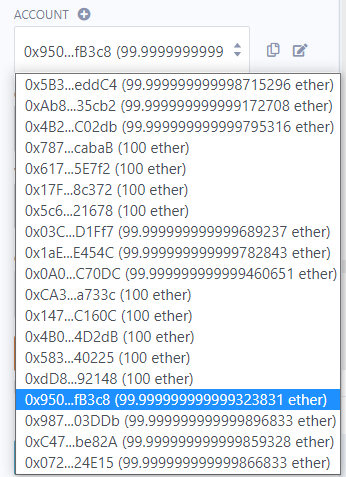
\includegraphics[width=.4\textwidth]{addresses}
		\captionof{figure}{\textit{List of addresses generated\\
			for the testnet with their value in Eth}}
		\label{addresses}
	\end{minipage}
}\\\\

For debugging purposes, the Remix\footnote{\url{https://remix-ide.readthedocs.io/en/latest}} environment, which is supported by the official Ethereum organization, offers graphical testing options on its web IDE. Figure \ref{interaction} shows this available options, where:

\begin{itemize}
	\item \underline{Orange buttons} \textit{voteAgainstAll}, \textit{voteNo}, and \textit{voteYes} are the three options available to vote for the referendum
	\item \underline{Blue button} \textit{getResult} reads the results from the blockchain and shows them encoded the following way:
	\begin{itemize}
		\item 0 is for the option \textit{yes}
		\item 1 is for the option \textit{no}
		\item 2 is for the option \textit{againstAll}
		\item 3 is the total amount of votes \textit{totalVotes}
	\end{itemize}
\end{itemize}

Reading variables from a contract deployed on the Ethereum blockchain does not consume any Ether, and can be done "for free" as many times as needed.\\

\makebox[0pt][l]{%
	\begin{minipage}{\textwidth}
		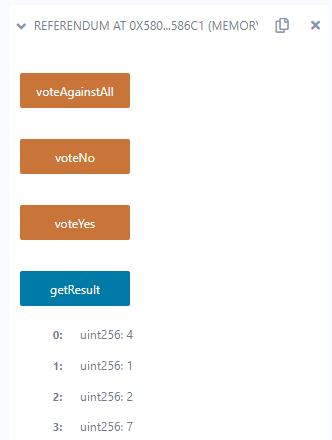
\includegraphics[width=.4\textwidth]{interaction}
		\captionof{figure}{\textit{Interactive menu for debugging\\
		the behavior of the smart contract}}
		\label{interaction}
	\end{minipage}
}\\\\

\subsection{Potential}

One of the good sides of any kind of online voting would be the reduction of costs it would suppose for the organizers (the administration, e.g.). Elections usually have a huge economic cost, as well as a complex logistics, and there would be no need to organize such an event.\\

In a situation of pandemic, voting online would reduce social interaction to virtually zero. There is no need to attend any physical place. In case of assistance during the election, all could be done remotely.\\

Voting from a computer or smartphone may seem convenient and more accessible for electors. It could even incentivize younger voters to do so, and promote a digital culture of doing things.\\

What's more, a blockchain-based voting system does not concern itself with the security of its Internet connection, because any hacker with access to a voter's terminal will not be able to affect other nodes, even if the identity and keys of this particular user are revealed.\\

Voters can effectively submit their vote without revealing their identity or political preferences to the public. The blockchain is in charge of protecting all voter's identity.\\

Such a technology would allow people to verify that their votes are recorded and counted correctly without compromising their anonymity. Moreover, anyone may be able to check the counting without breaking secrecy.

\subsection{Limitations and improvements}
\label{sec:limitations}

Distributed voting over a blockchain network sounds promising and would get us rid of many issues voting nowadays have. Nonetheless, there are claims made by  researchers\cite{ref:park} who say that blockchain-based voting could threaten democracy. Some security experts warn any internet-based election system is wide open to attack, regardless of the underlying infrastructure ---\textit{while current election systems are far from perfect, Internet and blockchain-based voting would greatly increase the risk of undetectable, nation-scale election failures}---.\\

In a centralised e-voting system, votes are stored in a database, but in a blockchain-based voting one, votes are variables stored over the network. A potential issue would be the case that the original smart contract had to be modified or updated for some reason. This would require to re-compile and deploy again, and this would suppose the loss of all the chain (and its stored votes) so far. There would be no way to recover the original votes like in a database, and could have catastrophic results for the election in course.\\

A similar issue would be the case in which the contract was not properly described and contains a point of failure. If this breaks in the middle of the voting process, the entire election would be compromised.\\

A way to prevent an issue like this would be to mimic a physical voting, where there are different ballots and one ballot being compromised does not mean the entire election compromised. A way to achieve this is by distributing the whole decentralized voting. This would be an implementation that consists of a master ballot contract that spawns multiple children, each containing the same proposal, but registers up to a total number of people living in a certain area. Registered voters receive their unique child ballot contract to vote with. This assignment can be done in many ways (based on geography, time registered, or just at random). When the voting ends, each child ballot contract will track its own votes itself and will report the result to the master ballot contract. The master ballot contract then consolidates and reports the final result.\\

In a permissioned blockchais like the referendum case there are often less severs when compared to larger pubic blockchains. Fewer servers increase the possibility of all of them becoming compromised.\\

Voters would have to be informed of what a blockchain-based election implies, given that if a voter loses their private key, they won’t be able to vote. If a malicious actor gains access to that key, they can vote for the user without anyone knowing.\\

Another downside of large-scale blockchains is the transaction time. Although Ethereum has faster transactions when compared to other platforms (such as Bitcoin), the transaction time would be too high in an election where there are more than 10M people expected to vote, which makes it not a good option.\\

Voting from a device such as a computer or smartphone may seem useful and a step forward in accessibility. However, studies have shown\cite{ref:park} that online voting may have little to no effect on turnout in practice, and it may even dis-encourage voting (Switzerland and Belgium). Studies from elections held in Estonia have also proved that turnout increase thanks to online voting may favor higher-income and higher-education demographics and can dis-encourage lower income citizens. Moscow also tried a blockchain-based voting system in September 2019. The government made the source code open and encouraged researchers to audit it. However, the system was shown to be gravely vulnerable and infeasible for large-scale elections.


\section{Conclusion and future work}

Blockchain is a disruptive technology that could easily promote the development of a larger ecosystem over time. Although implementing blockchain technology can bring many advantages to some sectors, it is the important to understand what it does well and what it doesn't do well.\\

Ethereum is a blockchain platform that completely revolutionizes the way transactions among peers are made. Given the powerful capabilities of smart contracts, it is possible to replace all existing ledger-based, physical standard contracts to improve transaction security, reduce costs and decentralize the architecture, with less dependence on servers. The applications are many, and it looks like just the beginning. In terms of use and development, Ethereum is evolving and becoming more mature with faster and a higher number of transactions compared to Bitcoin. One can believe that Ethereum will continue to grow and will remain one of the biggest players on the market for years.\\

For some companies and sectors, such as financial services and the supply chain industry, blockchain-based solutions will likely be implemented sooner than in many other industries. Blockchain has many promising applications in cryptocurrencies, where transactions among users are anonymous, although they are exposed to a high volatility in value and lack of regulation can be a problem. For digital identity, blockchain provides strong security and privacy when using it with online services, although there must be a central authority who issues the certificates at least once at the creation of the identity. For supercomputing applications, blockchain can be useful to divide computing requirements among peers, although the programming difficulty can be higher and the rewarding system a little tricky, so blockchain has to be thoroughly discussed before starting a project in supercomputing. The medical sector is one of the most benefited from blockchain as it has many uses: managing medical records, protecting and anonymizing healthcare data, or track drugs supply in pharmacies, e.g. Related to supply, blockchain has also a great application in supply chain, by increasing traceability, reduce costs and improve visibility and compliance with customers. And for crowdfunding, even though most platforms work on a centralized-basis, decentralization can be a good case study for studying how smart contracts work.\\

E-voting faces many challenges that has to enforce in order to be homologable to in-person voting, such as auditability, secrecy, or contestability. Blockchain can assure many of them, although it is not recommended to do after research results suggest. There are some flaws and vulnerabilities that can be dangerous for the election, and the proof it that no country in the world is using blockchain-based voting in their election system (beyond sporadic tests). Decentralized voting using blockchain is definitely not mature enough to be applicable to large-scale elections that imply a thorough scrutiny, although for smaller scale elections (company internal referendum, e.g.) could be feasible and an option to take into account. An alternative to blockchain would be to use centralized e-voting systems, which offer almost all advantages of blockchain (like voting from home using any device, or reduction of costs of setting physical ballots), without the flaws blockchain voting has.\\

Electronic, online, and blockchain-based voting systems are more vulnerable to serious failures than available paper-ballot-based alternatives. Adding new technologies to systems may create new potential for attacks. This is why it is not difficult to conclude that blockchain does not solve the fundamental security problems suffered by all electronic voting systems, and should be analyzed very deeply for such an application.\\

Some future work that follows the decentralized voting application studied, developed and deployed in this project would be to design the user interface that would simulate what a voter ---citizen--- would use, as well as to implement the authentication methods that are critical for ensuring that the correct user is voting on his behalf. This is something that could be achieved by using \textit{Web3}, a Javascript library that allows interacting with the smart contract, and an HTML web interface. Another improvement would be to design the distributed-decentralized voting ballots, as explained in section \ref{sec:limitations}. This would add complexity to the smart contract, but would make the polling more robust and less vulnerable to failure. It is fully feasible to do and Ethereum supports all these features.

\begin{thebibliography}{100}

%\bibitem{ref:miranda} 
%Victor Miranda Palacios. 
%\textit{Explorando la Blockchain de Ethereum y el desarrollo de smart contracts}. 
%Universitat Politècnica de Catalunya. Departament d'Enginyeria Telemàtica, 2018.

\bibitem{ref:soler} 
Laia Soler Izquierdo. 
\textit{Desarrollo de una DApp basada en Ethereum y React}. 
Universitat Politècnica de Catalunya. Departament d'Enginyeria Telemàtica, 2019.

\bibitem{ref:miras} 
Alberto Miras Gil. 
\textit{Deploying Ethereum infrastructure and DApps}. 
Universitat Politècnica de Catalunya. Departament d'Enginyeria Telemàtica, 2019.

\bibitem{ref:taule} 
Roger Taulé Buxadera. 
\textit{An Optimized System to Store Data on a Public Blockchain}. 
Universitat Politècnica de Catalunya. Departament d'Enginyeria Telemàtica, 2021.

\bibitem{ref:martin} 
Daniel Martín Martínez. 
\textit{Desenvolupament del vot descentralitzat}. 
Universitat Politècnica de Catalunya. Departament d'Arquitectura de Computadors, 2020

\bibitem{ref:klepatch} 
Julien Klepatch. 
\textit{Learn Ethereum DApps. Build a todo list with Solidity smart contract, Truffle, Javascript and Webpack}.
2019.

%\bibitem{ref:solomon} 
%Michael G. Solomon. 
%\textit{Ethereum for dummies}.
%Wiley, 2019.

\bibitem{ref:wu} 
Chun Chung Wu. 
\textit{Ethereum 101: Blockchain as Distributed Computation Platform}.
{\small \\\url{https://code.oursky.com/ethereum-blockchain-computation-platform}}

\bibitem{ref:park} 
Sunoo Park, Michael Specter, Neha Narula, Ronald L Rivest. 
\textit{Going from bad to worse: from Internet voting to blockchain voting}.

\bibitem{ref:isirova} 
Kateryna Isirova, Anastasiia Kiian, Mariia Rodinko, Alexandr Kuznetsov. 
\textit{Decentralized Electronic Voting System Based on Blockchain Technology Developing Principals}.

\bibitem{ref:buterin} 
Vitalik Buterin. 
\textit{Ethereum Whitepaper}.
{\small \\\url{https://ethereum.org/en/whitepaper}}

\end{thebibliography}

\end{multicols}

\end{document}
